\chapter{混合有限元法}
\section{混合方程}
混合有限元法基于混合变分原理,在分析的过程中同时选择两个基本未知函数,即节点位移函数和力函数。根据混合能量原理推导出混合方程。考虑混合变分问题:
存在$\boldsymbol \psi \in V$, $\lambda \in Q$,使
\begin{equation}
    \begin{aligned}
        a(\boldsymbol v, \boldsymbol \psi) + b(\boldsymbol v, \lambda) &= f(\boldsymbol v) \quad &\forall \boldsymbol v \in V \\
        b(\boldsymbol \lambda, q) &= g(\boldsymbol q) \quad &\forall q \in Q
    \end{aligned}
\end{equation}
其中$V, Q$为希尔伯特空间,定义为:
\begin{equation}
    V=\{\boldsymbol v \in H^1(\Omega)^2\;\vert\;\boldsymbol v = \boldsymbol g, \; \textrm{on} \; \Gamma_g\}
\end{equation}
\begin{equation}
    Q = \{q \in L^2(\Omega) \vert \int_{\Omega} q d\Omega = 0\}
\end{equation}
$a$是定义在 $V\times V\rightarrow$ 上的,$b$是定义在$V\times Q\rightarrow $ 上的连续双线性泛函, $f\in V'$($V$的对偶空间), $g\in Q'$($Q$的对偶空间)。
\section{不可压问题的混合离散法与罚函数法}               
\subsection{罚函数法}
考虑一个$n_d$维具有边界$\Gamma$的影响域$\Omega\in \mathbb R^{n_d}$,其中$\Gamma_t$和$\Gamma_g$分别表示其自然边界和本质边界,
且$\Gamma_t \cup \Gamma_g = \Gamma$, $\Gamma_t \cap \Gamma_g = \varnothing$。相应的混合控制方程由下式给出:
\begin{equation}\label{strong_penalty}
    \begin{cases}
        \nabla \cdot \boldsymbol \sigma + \boldsymbol b = \boldsymbol 0 & \mathrm{in} \; \Omega \\
        \boldsymbol \sigma \cdot \boldsymbol n = \boldsymbol t & \mathrm{on} \; \Gamma_t \\
        \boldsymbol u = \boldsymbol g & \mathrm{on} \; \Gamma_g \\
\end{cases}
\end{equation}
其中$\sigma$为应力张量,对于各向同性线弹性材料,可表示为:
\begin{equation}\label{stress_penalty}
    \boldsymbol \sigma(\boldsymbol u) = 3\kappa \boldsymbol \varepsilon^v(\boldsymbol u) + 2\mu \boldsymbol \varepsilon^d(\boldsymbol u) 
\end{equation}
式中$\boldsymbol \varepsilon^v$ 和 $\boldsymbol \varepsilon^d$ 为应变张量$\boldsymbol \varepsilon$的体积(膨胀)应变和偏应变部分,可表示为:
\begin{equation}
    \boldsymbol \varepsilon^v(\boldsymbol u) =\frac{1}{3} \nabla \cdot \boldsymbol u \; \boldsymbol 1, \quad
    \boldsymbol \varepsilon^d(\boldsymbol u) =\frac{1}{2}(\boldsymbol u \nabla + \nabla \boldsymbol u) - \boldsymbol \varepsilon^v, \quad
    \boldsymbol \varepsilon^v : \boldsymbol \varepsilon^d = 0
\end{equation}
$\kappa$, $\mu$ 为体积模量和剪切模量,与杨氏模量$E$和泊松比$\nu$之间存在如下关系式:
\begin{equation}\label{modulus}
    \kappa = \frac{E}{2(1-2\nu)}, \quad \mu = \frac{E}{2(1+\nu)}
\end{equation}
$\boldsymbol b$为$\Omega$中的体力, $\boldsymbol t$, $\boldsymbol g$ 分别为自然边界和本质边界上的牵引力和位移。

根据伽辽金法,位移$\boldsymbol u$可由下面的弱形式得到:
存在$\boldsymbol u \in V$使
\begin{equation}\label{weak_penalty}
\int_\Omega 2\mu \delta \boldsymbol \varepsilon^d : \boldsymbol \varepsilon^d d\Omega +
\int_\Omega 3\kappa \delta \boldsymbol \varepsilon^v : \boldsymbol \varepsilon^v d\Omega =
\int_{\Gamma_t} \delta \boldsymbol u \cdot \boldsymbol t d\Gamma + \int_\Omega \delta \boldsymbol u \cdot \boldsymbol b d\Omega, \quad
\forall \delta \boldsymbol u \in V
\end{equation}

在传统有限元法中,整个影响域$\Omega$由一组具有节点$\{\boldsymbol x_I\}_{I=1}^{n_u}$的构造网格离散\cite{hughes2000},其中$n_u$是节点的数量。
位移$u$及其变分$\delta u $可通过$x_I$处的节点系数和形函数进行近似:
\begin{equation}\label{u_h}
    \boldsymbol u_h(\boldsymbol x) = \sum_{I=1}^{n_u} N_I(\boldsymbol x) \boldsymbol u_I, \quad
    \delta \boldsymbol u_h(\boldsymbol x) = \sum_{I=1}^{n_u} N_I(\boldsymbol x) \delta \boldsymbol u_I
\end{equation}
其中$N_I$和$u_I$分别为节点$x_I$处的形函数和节点系数张量。将式\eqref{u_h}代入到弱形式\eqref{weak_penalty}中可得下列的里兹-伽辽金变分方程:
存在 $\boldsymbol u_h \in V_h$,使
\begin{equation}\label{ritz_penalty}
\int_\Omega 2\mu \delta \boldsymbol \varepsilon^d_h : \boldsymbol \varepsilon^d_h d\Omega +
\int_\Omega 3\kappa \delta \boldsymbol \varepsilon^v_h : \boldsymbol \varepsilon^v_h d\Omega =
\int_{\Gamma_t} \delta \boldsymbol u_h \cdot \boldsymbol t d\Gamma + \int_\Omega \delta \boldsymbol u_h \cdot \boldsymbol b d\Omega, \quad
\forall \delta \boldsymbol u_h \in V_h
\end{equation}
其中近似空间$V_h \subseteq V$,
\begin{equation}
    V_h = \{\boldsymbol v_h \in (\mathrm{span}\{N_I\}_{I=1}^{n_u})^2 \vert \boldsymbol v^h = \boldsymbol g,\; \mathrm{on} \; \Gamma_g\}
\end{equation}
根据$\delta u_h$的任意性,通过消除$\delta u_I$,上述方程可以简化为以下离散控制方程:
\begin{equation}\label{equilibrium_penalty}
    (2\mu\boldsymbol K^d + 3\kappa\boldsymbol K^v) \boldsymbol d^u = \boldsymbol f
\end{equation}
式中,体积刚度矩阵$\boldsymbol K^v$ 和偏刚度矩阵 $\boldsymbol K^d$的分量分别为:
\begin{equation}\label{stiffness_vol}
    \boldsymbol K^v_{IJ}= \int_{\Omega} \boldsymbol B^{vT}_I \boldsymbol B^v_J d\Omega
\end{equation}
\begin{equation}
    \boldsymbol K^d_{IJ}= \int_{\Omega} \boldsymbol B^{dT}_I \boldsymbol B^d_J d\Omega
\end{equation}
力向量$\boldsymbol f$的分量为:
\begin{equation}
    \boldsymbol f_I = \int_{\Gamma_t} N_I \boldsymbol t d\Gamma + \int_{\Omega} N_I \boldsymbol b d\Omega
\end{equation}
$\boldsymbol d^u$ 是包含 $\boldsymbol u_I$的系数向量。

从式\eqref{modulus}可以得出,对于几乎不可压缩的材料,当$\nu \rightarrow 0.5$, $\kappa \rightarrow \infty$。
因此式\eqref{equilibrium_penalty}中的体积刚度矩阵$\boldsymbol K^v$可视作一种强制使用的罚函数法使得体积变形为$0$,即$\nabla \cdot \boldsymbol u = 0$,而体积模量$\kappa$可视作罚因子。
由于这种情况,使用传统有限元法会产生严重的体积锁定,就是所谓的体积自锁。通过减少体积刚度矩阵中的积分点数量,可以达到缓解体积自锁的目的。
为了清晰起见,将数值积分代入式\eqref{ritz_penalty}
\begin{equation}
    \int_\Omega 3\kappa \delta \boldsymbol \varepsilon^v_h : \boldsymbol \varepsilon^v_h d\Omega \approx
    \sum_{C=1}^{n_e}\sum_{G=1}^{n_g} 3\kappa \nabla \cdot \delta \boldsymbol u_h(\boldsymbol x_G) \nabla \cdot \boldsymbol u_h(\boldsymbol x_G) w_G
\end{equation}
式\eqref{stiffness_vol}中的体积刚度矩阵$\boldsymbol K^v$的分量可以改写为:
\begin{equation}
    \boldsymbol K^v_{IJ} \approx \bar{\boldsymbol K}^v_{IJ} = \sum_{C=1}^{n_e}\sum_{G=1}^{n_g} \boldsymbol B^{vT}_I(\boldsymbol x_G) \boldsymbol B_J^v(\boldsymbol x_G) w_G
\end{equation}

其中,$\boldsymbol x_G$和$w_G$分别为积分点的位置和权重。$n_g$是每个单元中积分点的数量,因此总的积分点数量为$n_c \times n_g$。
与传统的完全积分法相比,缩减积分法使用积分点的数量更少。例如,传统四边形单元使用$2\times2$高斯积分点作为全积分,全积分意味着可以更加精确的计算刚度矩阵。而对于缩减积分,积分点的数量从4个减少到1个。

\subsection{混合离散法}
缓解体积自锁的另一种方法是混合离散法。在这种方法中,压力通过另一种方式近似:
\begin{equation}\label{stress_mix}
    \boldsymbol \sigma(\boldsymbol u, p) = p \boldsymbol 1 + 2\mu \boldsymbol \varepsilon^d(\boldsymbol u)
\end{equation}
混合离散法的强形式可以改写为:
\begin{equation}\label{strong_mix}
    \begin{cases}
        \nabla \cdot \boldsymbol \sigma + \boldsymbol b = \boldsymbol 0 & \mathrm{in} \; \Omega \\
        \frac{p}{\kappa} + \nabla \cdot \boldsymbol u = 0 & \mathrm{in} \; \Omega \\
        \boldsymbol \sigma \cdot \boldsymbol n = \boldsymbol t & \mathrm{on} \; \Gamma_t \\
        \boldsymbol u = \boldsymbol g & \mathrm{on} \; \Gamma_g \\
    \end{cases}
\end{equation}
其中$p\in Q$。

根据伽辽金公式,弱形式可以定义为:
存在$\boldsymbol u \in V$, $p \in Q$,使
\begin{equation}
    \begin{aligned}
        a(\boldsymbol v, \boldsymbol u) + b(\boldsymbol v, p) &= f(\boldsymbol v) \quad &\forall \boldsymbol v \in V \\
        b(\boldsymbol u, q) &= \boldsymbol 0 \quad &\forall q \in Q
    \end{aligned}
\end{equation}
在弹性问题中,它们具有以下形式:
\begin{equation}
    a(\boldsymbol v, \boldsymbol u) = \int_\Omega \nabla^s \boldsymbol v : \nabla^s \boldsymbol u d\Omega
\end{equation}
\begin{equation}
    b(\boldsymbol v, p) = \int_\Omega \nabla \cdot \boldsymbol v p d\Omega
\end{equation}
\begin{equation}
    b(\boldsymbol u, q) = \int_\Omega q(\nabla \cdot \boldsymbol u - \frac{1}{3\kappa} p)d\Omega
\end{equation}
\begin{equation}
    f(\boldsymbol v) = \int_{\Gamma_t} \boldsymbol v \cdot \boldsymbol t d\Gamma + \int_{\Omega} \boldsymbol v \cdot \boldsymbol b d\Omega
\end{equation}

在传统的混合离散法中,压力$p$由不同的控制节点离散,即位移节点$\{\boldsymbol x_I\}_{I=1}^{n_d}$和压力节点$\{\boldsymbol x_K\}_{K=1}^{n_p}$,其中$n_d$和$n_p$分别为位移节点和压力节点的总数。
于是近似位移$\boldsymbol u_h$和近似压力$p_h$可以表示为:
\begin{equation}\label{u_h_mix}
    \boldsymbol u_h(\boldsymbol x) = \sum_{I=1}^{n_d} N^d_I(\boldsymbol x) \boldsymbol u_I, \quad
    \delta \boldsymbol u_h(\boldsymbol x) = \sum_{I=1}^{n_d} N^d_I(\boldsymbol x) \delta \boldsymbol u_I
\end{equation}
\begin{equation}\label{p_h_mix}
    p_h(\boldsymbol x) = \sum_{K=1}^{n_p} N^p_K(\boldsymbol x) p_K, \quad
    \delta p_h(\boldsymbol x) = \sum_{K=1}^{n_p} N^p_K(\boldsymbol x) \delta p_K
\end{equation}
式中,$p_K$是节点系数,$N^d_I$、$N^p_K$是对应的形函数。相应的里兹-伽辽金变分方程如下:
存在$\boldsymbol u_h \in V_h$, $p_h \in Q_h$使
\begin{equation}
    \begin{aligned}
        a(\boldsymbol v_h, \boldsymbol u_h) + b(\boldsymbol v_h, p_h) &= f(\boldsymbol v_h) \quad &\forall \boldsymbol v_h \in V_h \\
        b(\boldsymbol u_h, q_h) &= \boldsymbol 0 \quad &\forall q_h \in Q_h
    \end{aligned}
\end{equation}
即
\begin{subequations}\label{ritz_mix}
\begin{alignat}{2}
\label{ritz_mix_1}
\int_\Omega 2\mu \delta \boldsymbol \varepsilon^d_h : \boldsymbol \varepsilon^d_h d\Omega +
\int_\Omega \nabla \cdot \delta \boldsymbol u_h p_h d\Omega &=
\int_{\Gamma_t} \delta \boldsymbol u_h \cdot \boldsymbol t d\Gamma + \int_\Omega \delta \boldsymbol u_h \cdot \boldsymbol b d\Omega, \quad
&\forall \delta \boldsymbol u_h \in V_h \\
\label{ritz_mix_2}
\int_\Omega \delta p_h \nabla \cdot \boldsymbol u_h d\Omega - \int_\Omega \frac{1}{3\kappa} \delta p_h p_h d\Omega &= 0, &\forall \delta p_h \in Q_h
\end{alignat}
\end{subequations}

根据$u_h$和$p_h$的任意性,式\eqref{ritz_mix}可得到如下离散控制方程:
\begin{equation}\label{equilibrium_mix}
    \begin{bmatrix}
        2\mu\boldsymbol K^{uu} & \boldsymbol K^{up} \\ (\boldsymbol K^{up})^T & -\frac{1}{3\kappa}\boldsymbol K^{pp}
    \end{bmatrix}
    \begin{Bmatrix}
        \boldsymbol d^u \\ \boldsymbol d^p 
    \end{Bmatrix} =
    \begin{Bmatrix}
        \boldsymbol f \\ \boldsymbol 0 
    \end{Bmatrix}
\end{equation}
式中$\boldsymbol K^{uu} = \boldsymbol K^d$. 

由式\eqref{equilibrium_mix}离散控制方程中的第二个等式,系数向量$d^p$可用$d^u$表示:
\begin{equation}
    \boldsymbol d^p = 3\kappa(\boldsymbol K^{pp})^{-1} (\boldsymbol K^{up})^T \boldsymbol d^u
\end{equation}
将上式代入到式\eqref{equilibrium_mix}的第一个等式中可得:
\begin{equation}\label{equilibrium_projection}
    \begin{split}
        &(2\mu\underbrace{\boldsymbol K^{uu}}_{\boldsymbol K^d} + 3\kappa \underbrace{\boldsymbol K^{up}(\boldsymbol K^{pp})^{-1}(\boldsymbol K^{up})^{T}}_{\tilde{\boldsymbol K}^v}) \boldsymbol d^u = \boldsymbol f \\
        \Rightarrow\;& (2\mu \boldsymbol K^d + 3\kappa \tilde{\boldsymbol K}^v) = \boldsymbol f
    \end{split}
\end{equation}

\subsection{罚函数法和混合方法的等价性}
从混合离散法的弱形式\eqref{ritz_mix_2}或离散方程\eqref{equilibrium_projection}中可以看出,压力$p_h$的解是$3\kappa \nabla \cdot \boldsymbol u_h$的一个正交投影。
令$P_h: V_h \rightarrow P_h(V_h)$ 使得 $P_h(V_h) \subseteq Q_h$, 其中 $P_h(V_h) = \textrm{Im}\:P_h$ 是线性算子$P_h$的虚部 \cite{philippeg.2013}. 
在这种情况下, $p_h = P_h (3\kappa \nabla \cdot \boldsymbol u_h) = 3\kappa \tilde \nabla \cdot \boldsymbol u_h$,式\eqref{ritz_mix_2}可以改写为:
\begin{equation}
    \int_\Omega q_h(\nabla \cdot \boldsymbol u_h - \tilde \nabla \cdot \boldsymbol u_h) d\Omega = 0, \quad \forall q_h \in Q_h
\end{equation}
相应的,弱形式体积部分变为:
\begin{equation}\label{projection_mixed}
    \begin{split}
        \int_\Omega \nabla \cdot \delta \boldsymbol u_h p_h d\Omega &= \underbrace{\int_\Omega (\nabla \cdot \boldsymbol u_h - \tilde \nabla \cdot \delta \boldsymbol u_h) p_h d\Omega}_0 + \int_\Omega \tilde \nabla \cdot \delta \boldsymbol u_h \underbrace{p_h}_{\tilde \nabla \cdot \boldsymbol u_h} d\Omega \\
        &= \int_\Omega 3\kappa \tilde \nabla \cdot \delta \boldsymbol u_h \tilde \nabla \cdot \boldsymbol u_h d\Omega \\
    \end{split}
\end{equation}
里兹-伽辽金变分方程变为:
存在$\boldsymbol u_h \in V_h$使
\begin{equation}
    \int_\Omega 2\mu \delta \boldsymbol \varepsilon^d_h : \boldsymbol \varepsilon^d_h d\Omega +
    \int_\Omega 3\kappa \tilde \nabla \cdot \delta \boldsymbol u_h \tilde \nabla \cdot \boldsymbol u_h d\Omega =
    \int_{\Gamma_t} \delta \boldsymbol u_h \cdot \boldsymbol t d\Gamma + \int_\Omega \delta \boldsymbol u_h \cdot \boldsymbol b d\Omega, \quad \forall \boldsymbol u_h \in V_h
\end{equation}

相比之下,对于罚函数法,缩减积分也可以被视作一种投影。设$\varrho_i$为正交多项式,
\begin{equation}
    \int_{\Omega_C} \varrho_i \varrho_j d\Omega = 
    \begin{cases}
        J_C w_i  & i = j \\
        0 & i \ne j
    \end{cases}
\end{equation}
正交插值 $T^{k}: V \rightarrow W^{k}$,其中 $W^{k}$ 是由$k$个正交多项式构成的插值空间:
\begin{equation}
    W^{k}:= \mathrm{span}\{\varrho_i \}_{i=1}^{k}
\end{equation}
对于传统高斯积分方案,$\varrho_i(\boldsymbol x_j) = \delta_{ij}$, $\boldsymbol x_j$是积分点的位置。体积应变可以通过正交插值法表示为:
\begin{equation}
    \nabla \cdot \boldsymbol u_h(\boldsymbol x) \approx \bar \nabla \cdot \boldsymbol u_h(\boldsymbol x) = \sum_{G=1}^{n_g} \varrho_G(\boldsymbol x) \nabla \cdot \boldsymbol u_h(\boldsymbol x_G), \quad \nabla \cdot \boldsymbol u_h(\boldsymbol x_G) = \bar \nabla \cdot \boldsymbol u_h(\boldsymbol x_G)
\end{equation}
而积分点被视为插值系数。虽然积分点的总数$n_g$低于完全积分,这意味着 $\nabla \cdot \boldsymbol u_h$ 投影到子空间。
\begin{equation}\label{projection_penalty}
    \begin{split}
        \int_\Omega 3\kappa \bar \nabla \cdot \delta \boldsymbol u_h \bar \nabla \cdot \boldsymbol u_h d\Omega
        &= \sum_{C=1}^{n_e} \sum_{G,L=1}^{n_g} 3\kappa \nabla \cdot \delta \boldsymbol u_h(\boldsymbol x_G) \nabla \cdot \boldsymbol u_h(\boldsymbol x_L) \int_\Omega \varrho_G \varrho_L d\Omega  \\
        &= \sum_{C=1}^{n_e} \sum_{G=1}^{n_g} 3\kappa \nabla \cdot \delta \boldsymbol u_h(\boldsymbol x_G) \nabla \cdot \boldsymbol u_h(\boldsymbol x_G) J_C w_G \\
    \end{split}
\end{equation}

通过对比式\eqref{projection_penalty}和式\eqref{projection_mixed},罚函数法实际上与混合离散法等价,两种方法都可以用投影的方式来描述。

\section{中厚板问题的混合离散法与罚函数法}      
\subsection{罚函数法}
考虑如图\ref{mindlin_picture}所示中厚板,其中中板厚为$h$,$\Omega$为板中面。在Mindlin假设下,中厚板考虑横向剪切变形,相应的混合控制方程由下式给出:
\begin{equation}\label{strong_mindlin}
    \begin{cases}
        M_{\alpha\beta,\beta} - Q_\alpha = 0 & \textrm{in}\; \Omega \\
        Q_{\alpha,\alpha} + \bar q = 0 & \textrm{in}\; \Omega \\    Q_\alpha n_\alpha = \bar Q & \textrm{on}\; \Gamma_Q \\
        M_{\alpha\beta} n_\beta = \bar M_\alpha & \textrm{on}\; \Gamma_M \\
        \varphi_\alpha = \bar \varphi_\alpha & \textrm{on}\; \Gamma_\varphi \\
        w = \bar w & \textrm{on}\; \Gamma_w \\
    \end{cases}
\end{equation}
式中,$M_{\alpha \beta}$ 可表示弯矩张量$\pmb{M}$ 的弯曲或扭转部分的分量,$\bar{q}$ 为垂直于板中面的分布荷载;
$\Gamma_w$和$\Gamma_\varphi$为本质边界条件,$\bar{w}$和$\bar{\varphi}_\alpha$分别为本质边界条件上给定的挠度和转角;
$\Gamma_Q$ 和$\Gamma_M$ 为自然边界条件,$\bar Q$和$\bar{M}_{\alpha}$ 为自然边界上的等效剪力和法向弯矩;
$n_\alpha$为边界上外法线方向$\pmb{n}$的分量。
\begin{figure}[H]
    \centering 
        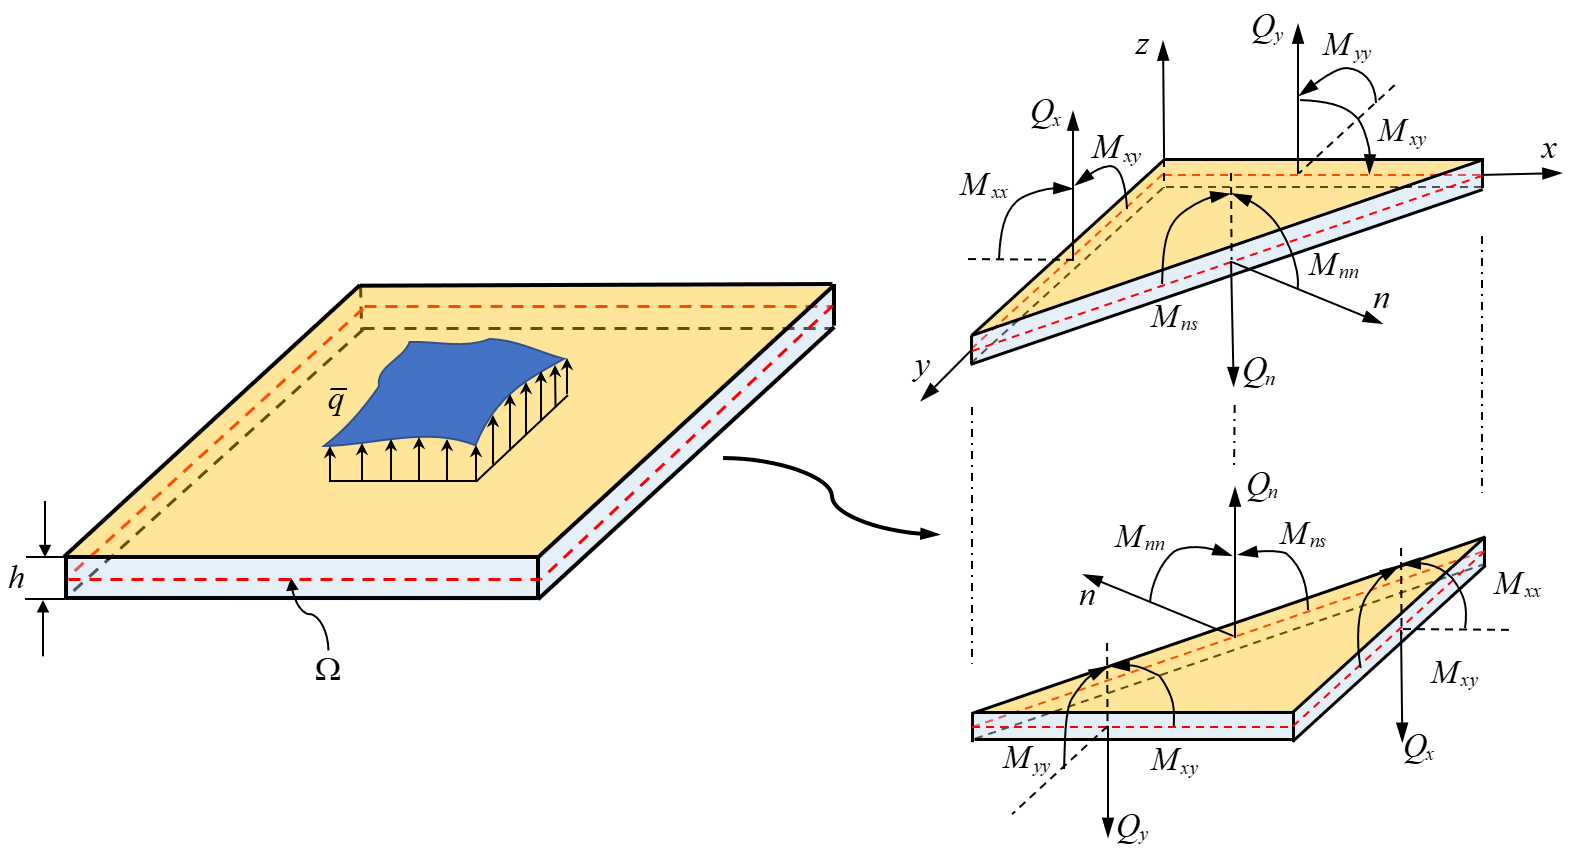
\includegraphics[scale=0.5]{figures/shearlocking/Mindlinplate.png}
        \caption{中厚板运动学及边界条件}\label{mindlin_picture}
\end{figure}

在平面应力假设下,当中厚板为线弹性各同向性材料时,其本构关系为:
\begin{equation} 
    \begin{split}
    M_{\alpha \beta}=-\frac{h^3}{12}D_{\alpha \beta \gamma\eta}\kappa_{\gamma\eta}=\frac{h^3}{12}D_{\alpha \beta \gamma\eta}\varphi_{\gamma,\eta}
    \end{split}
\end{equation}
\begin{equation} 
    \begin{split}
    Q_{\alpha}=k\frac{Eh}{2(1+\nu)}\gamma_\beta=kGh(-\varphi_\beta+w_{,\beta})
    \end{split}
\end{equation}
其中$k$为剪切修正系数,$\kappa_{\alpha\beta}$为曲率张量$\pmb\kappa$的分量,$\gamma_\alpha$为剪切应变矢量$\pmb\gamma$的分量,表达式为:
\begin{equation} 
    \kappa_{\alpha\beta}=-\varphi_{\alpha,\beta},\quad\gamma_\alpha=-\varphi_\alpha+w_{,\alpha}
\end{equation}
其中$D_{\alpha \beta \gamma\eta}$为在平面应力假设下四阶弹性张量的分量,表达式为:
\begin{equation} 
    D_{\alpha \beta \gamma\eta}=\frac{E}{1-\nu^2}(\nu\delta_{\alpha\beta}\delta_{\gamma\eta}+\frac{1}{2}(1-\nu)(\delta_{\alpha\gamma}\delta_{\beta\eta}+\delta_{\alpha\eta}\delta_{\beta\gamma}))
\end{equation}

根据最小势能原理,强形式\eqref{strong_mindlin}所对应的势能泛函表达式为: 
\begin{equation}\label{potential_energy}
    \begin{split} 
        \Pi(w,\boldsymbol{\varphi})&=\frac{1}{2}\int_{\Omega}\kappa_{\alpha\beta}M_{\alpha\beta}d\Omega+\frac{1}{2}\int_{\Omega}\gamma_{\alpha}Q_{\alpha}d\Omega\\
        &+\int_{\Gamma_{M}}\varphi_{\alpha}{\bar{M}_{\alpha}}d\Gamma-\int_{\Gamma_{Q}}{w}\bar {Q}d\Gamma-\int_{\Omega} w\bar{q}d\Omega
    \end{split}
\end{equation}
对式\eqref{potential_energy}进行变分可得弱形式:
存在$(w,\varphi_{\alpha})\in V$,使
\begin{equation}\label{weak_penalty_mindlin}
    \begin{split} 
        &\int_{\Omega}\delta\kappa_{\alpha\beta}M_{\alpha\beta}d\Omega+\int_{\Omega}\delta\gamma_{\alpha}Q_{\alpha}d\Omega=\\
        &-\int_{\Gamma_{M}}\delta\varphi_{\alpha}{\bar{M}_{\alpha}}d\Gamma+\int_{\Gamma_{Q}}{\delta{w}}\bar {Q}d\Gamma+\int_{\Omega} \delta{w}\bar{q}d\Omega,\quad \forall(\delta w,\delta\varphi_{\alpha}) \in V
    \end{split}
\end{equation}

在传统有限元法中,整个影响域$\Omega$由一组具有节点$\{\boldsymbol x_I\}_{I=1}^{n_u}$的构造网格离散,其中$n_u$是节点的数量。
挠度$w$及其变分$\delta w $,转角$\varphi$及其变分$\delta \varphi $可通过$x_I$处的节点系数和形函数进行近似:
\begin{equation}
    w_h(\boldsymbol x) = \sum_{I=1}^{n_u} N_I(\boldsymbol x) w_I, \quad \delta w_h(\boldsymbol x) = \sum_{I=1}^{n_u} N_I(\boldsymbol x) \delta w_I
\end{equation}
\begin{equation}
    \varphi_{\alpha h}(\boldsymbol x) = \sum_{I=1}^{n_u} N_I(\boldsymbol x) \varphi_{\alpha I}, \quad \delta \varphi_h(\boldsymbol x) = \sum_{I=1}^{n_u} N_I(\boldsymbol x) \delta \varphi_{\alpha I}
\end{equation}
其中,$N_I$为节点$x_I$处的形函数,和$w_I$和$\varphi_{\alpha I}$节点系数张量。
相应的近似曲率$\pmb\kappa_h$和近似剪切应变$\pmb\gamma_h$可表示为:
\begin{equation}
    \boldsymbol\kappa_h = 
    \begin{Bmatrix}
        \kappa^h_{11} \\ \kappa^h_{22} \\ 2\kappa^h_{12} 
    \end{Bmatrix} = -\sum_{I=1}^{n_u}
    \begin{bmatrix}
        0 & N_{I,1} & 0 \\ 0 & 0 & N_{I,2} \\ 0 & N_{I,2} & N_{I,1}
    \end{bmatrix}
    \begin{Bmatrix}
        w_I \\ \varphi_{1I} \\ \varphi_{2I}
    \end{Bmatrix} = - \sum_{I=1}^{n_u} \boldsymbol B^b_I \boldsymbol d_I
\end{equation}
\begin{equation}
    \boldsymbol\gamma_h = 
    \begin{Bmatrix}
        \gamma^h_1 \\ \gamma^h_2
    \end{Bmatrix} = \sum_{I=1}^{n_u}
    \begin{bmatrix}
        N_{I,1} & N_I & 0 \\
        N_{I,2} & 0 & N_I
    \end{bmatrix}
    \begin{Bmatrix}
        w_I \\ \varphi_{1I} \\ \varphi_{2I}
    \end{Bmatrix} = \sum_{I=1}^{n_u} \boldsymbol B^s_I \boldsymbol d_I
\end{equation}
\begin{equation}\label{kappa_h}
    \delta\boldsymbol\kappa_h = - \sum_{I=1}^{n_u} \boldsymbol B^b_I \delta\boldsymbol d_I ,\quad \delta\boldsymbol\gamma_h = \sum_{I=1}^{n_u} \boldsymbol B^s_I \delta\boldsymbol d_I
\end{equation}
将式\eqref{kappa_h}代入到弱形式\eqref{weak_penalty_mindlin}可得下列变分方程:
存在$(w_h,\boldsymbol{\varphi}_{\alpha h})\in V_h$,使
\begin{equation}\label{ritz_penalty_mindlin}
    \begin{split} 
        &\int_{\Omega}\delta\kappa^h_{\alpha\beta}M_{\alpha\beta}d\Omega+\int_{\Omega}\delta\gamma^h_{\alpha}Q_{\alpha}d\Omega=\\
        &-\int_{\Gamma_{M}}\delta\varphi_{\alpha h}{\bar{M}_{\alpha}}d\Gamma+\int_{\Gamma_{Q}}{\delta{w_h}}\bar {Q}d\Gamma+\int_{\Omega} \delta{w}\bar{q}d\Omega,\quad \forall(\delta w_h,\delta\varphi_{\alpha h}) \in V_h
    \end{split}
\end{equation}

根据$\pmb\kappa_h$和$\pmb\gamma_h$的任意性,上述方程可简化为如下离散控制方程:
\begin{equation}
    (\boldsymbol K^b + \boldsymbol K^s) \boldsymbol d = \boldsymbol f
\end{equation}
其中弯曲刚度矩阵$\boldsymbol K^b$和剪切刚度矩阵$\boldsymbol K^s$是具有以下分量:
\begin{subequations}\label{stiffness_mindlin}
    \begin{alignat}{2}
    \label{stiffness_bending}
    \boldsymbol K^b_{IJ} = \frac{h^3}{12} \int_\Omega \boldsymbol B^{bT}_I \boldsymbol D \boldsymbol B^b_J d\Omega\\
    \label{stiffness_shear}
    \boldsymbol K^s_{IJ} = h \int_\Omega \boldsymbol B^{sT}_I kG \boldsymbol B^s_J d\Omega
    \end{alignat}
\end{subequations}
式中$\pmb{D}$为平面应力弹性矩阵,$\pmb{f}$为力矢量,其分量具有以下形式:
\begin{equation}
    \boldsymbol f_I = \int_{\Gamma_Q} N_I \bar{\boldsymbol Q} d\Gamma - \int_{\Gamma_M} N_I \bar{\boldsymbol M} d\Gamma + \int_\Omega N_I \bar{\boldsymbol q} d\Omega
\end{equation}
其中:
\begin{equation}
    \bar{\boldsymbol Q} =  
    \begin{Bmatrix}
        \bar Q \\ 0 \\ 0
    \end{Bmatrix},
        \bar{\boldsymbol M} =
    \begin{Bmatrix}
        0 \\ \bar M_1 \\ \bar M_2
    \end{Bmatrix},
        \bar{\boldsymbol q} =
    \begin{Bmatrix}
        \bar q \\ 0 \\ 0
    \end{Bmatrix}
\end{equation}

从式\eqref{stiffness_mindlin},对于考虑厚度方向变形的中厚板,当厚度$h$减少时,剪切刚度远大于弯曲刚度,使得板弯曲变形为$0$,而产生虚假的横向剪切应力。
由于这种情况,使用传统有限元法会产生严重的剪切锁定,就是所谓的剪切自锁。通过减少剪切刚度矩阵中积分点的数量,可以缓解剪切自锁。将数值积分代入式\eqref{ritz_penalty_mindlin}
\begin{equation}
    \int_{\Omega}\delta\gamma^h_{\alpha}Q_{\alpha}d\Omega \approx
    \sum_{C=1}^{n_e}\sum_{G=1}^{n_g} h \delta\gamma^h_{\alpha}(\boldsymbol x_G) kG \delta\gamma^h_{\alpha}(\boldsymbol x_G) w_G
\end{equation}
式\eqref{stiffness_shear}中的剪切刚度矩阵$\boldsymbol K^s$的分量可以改写为:
\begin{equation}
    \boldsymbol K^s_{IJ} \approx \bar{\boldsymbol K}^s_{IJ} = \sum_{C=1}^{n_e}\sum_{G=1}^{n_g} h\boldsymbol B^{sT}_I(\boldsymbol x_G) \boldsymbol B_J^s(\boldsymbol x_G) w_G
\end{equation}

\subsection{混合离散法}
为了缓解厚度减小引起的剪切自锁,引入与挠度和转角无关的剪切应力$\pmb{Q}$,根据最小势能原理,势能泛函的表达式可更改为:
\begin{equation}\label{potential_energy_mixed}
\begin{split} 
    \Pi(w,\boldsymbol{\varphi},\boldsymbol{Q})&=\int_{\bar\Omega}\frac{1}{2}\varepsilon_{ij}\sigma_{ij} d\Omega+\frac{1}{2}\int_{\Omega}Q_{\alpha}(\gamma_{\alpha}-\frac{Q_{\alpha}}{kGh})d\Omega-\int_{\Gamma^{t}} u_{i}t_{i}d\Gamma-\int_{\Omega} u_{i}b_{i}d\Omega\\
    &=\frac{1}{2}\int_{\Omega}(\kappa_{\alpha \beta}M_{\alpha \beta}+\gamma_{\alpha}Q_{\alpha})d\Omega+\frac{1}{2}\int_{\Omega}Q_{\alpha}(\gamma_{\alpha}-\frac{Q_{\alpha}}{kGh})d\Omega\\
    &+\int_{\Gamma_{M}}\pmb\varphi_{\alpha}{\bar{M}_{\alpha}}d\Gamma-\int_{\Gamma_{Q}}{w}\bar {Q}d\Gamma-\int_{\Omega} w\bar{q}d\Omega
\end{split}
\end{equation}
对式\eqref{potential_energy_mixed}进行变分可得弱形式:
\begin{equation} 
    \begin{split}
    &\delta\Pi(w,\boldsymbol\varphi,\boldsymbol{Q})\\
    &=\int_{\Omega}\delta\kappa_{\alpha \beta}M_{\alpha \beta}d\Omega+\frac{1}{2}\int_{\Omega}\delta\gamma_{\alpha}Q_{\alpha}d\Omega+\frac{1}{2}\int_{\Omega}\gamma_{\alpha}\delta{Q}_{\alpha}d\Omega+\frac{1}{2}\int_{\Omega}\delta\gamma_{\alpha}Q_{\alpha}d\Omega\\
    &+\frac{1}{2}\int_{\Omega}\gamma_{\alpha}\delta{Q}_{\alpha}d\Omega-\int_{\Omega}\frac{\delta{Q}_{\alpha}{Q}_{\alpha}}{kGh}d\Omega+\int_{\Gamma_{M}}\delta\varphi_{\alpha}{{\bar M}_{\alpha}}d\Gamma-\int_{\Gamma_{Q}}\delta{w}{\bar Q}d\Gamma+\int_{\Omega} \delta{w}\bar{q}d\Omega\\
    &=\int_{\Omega}\delta\kappa_{\alpha \beta}M_{\alpha \beta}d\Omega+\int_{\Omega}\delta\gamma_{\alpha}Q_{\alpha}d\Omega+\int_{\Omega}\gamma_{\alpha}\delta{Q}_{\alpha}d\Omega-\int_{\Omega}\frac{\delta{Q}_{\alpha}{Q}_{\alpha}}{kGh}d\Omega+\int_{\Gamma_{M}}\delta\varphi_{\alpha}{\boldsymbol{\bar M}_{\boldsymbol{\alpha}}}d\Gamma\\
    &-\int_{\Gamma_{Q}}\delta{w}{\bar Q}d\Gamma+\int_{\Omega} \delta{w}\bar{q}d\Omega\\
    &=0
    \end{split}
\end{equation}
由上式弱形式可以定义为:
存在$\boldsymbol u \in V$, $p \in Q$,使
\begin{equation}
    \begin{aligned}
        a(\boldsymbol v, \boldsymbol u) + b(\boldsymbol v, p) &= f(\boldsymbol v) \quad &\forall \boldsymbol v \in V \\
        b(\boldsymbol u, q) &= \boldsymbol 0 \quad &\forall q \in Q
    \end{aligned}
\end{equation}
即:
\begin{equation}\label{mindlin_weak1}
    \int_{\Omega}\delta\kappa_{\alpha \beta}M_{\alpha \beta}d\Omega+\int_{\Omega}\delta\gamma_{\alpha}Q_{\alpha}d\Omega=\int_{\Gamma_{Q}}\delta{w}{\bar Q}d\Gamma-\int_{\Omega} \delta{w}\bar{q}d\Omega-\int_{\Gamma_{M}}\delta\varphi_{\alpha}{{\bar M}_{\alpha}}d\Gamma
\end{equation}
\begin{equation}\label{mindlin_weak2}
    \int_{\Omega}\gamma_{\alpha}\delta{Q}_{\alpha}d\Omega-\int_{\Omega}\frac{\delta{Q}_{\alpha}{Q}_{\alpha}}{kGh}d\Omega=0
\end{equation}
对挠度、转角和剪切应力采用混合离散的方式进行近似。近似剪切应力$Q_\alpha^h$可表示为:
\begin{equation}\label{Q_h}
    Q^h_\alpha(\boldsymbol x) = \sum_{K=1}^{n_q} N^q_K(\boldsymbol x) q_{\alpha K},\quad \delta Q^h_\alpha(\boldsymbol x) = \sum_{K=1}^{n_q} N^q_K(\boldsymbol x) \delta q_{\alpha K}
\end{equation}
其中$q_{\alpha K}$是节点系数,$N^q_K$是对应的形函数。相应的里兹-伽辽金变分方程如下:
存在$\boldsymbol u_h \in V_h$, $p_h \in Q_h$使
\begin{equation}
    \begin{aligned}
        a(\boldsymbol v_h, \boldsymbol u_h) + b(\boldsymbol v_h, p_h) &= f(\boldsymbol v_h) \quad &\forall \boldsymbol v_h \in V_h \\
        b(\boldsymbol u_h, q_h) &= \boldsymbol 0 \quad &\forall q_h \in Q_h
    \end{aligned}
\end{equation}
即:
\begin{equation}\label{mindlin_ritz1}
    \int_{\Omega}\delta\kappa^h_{\alpha \beta}M_{\alpha \beta}d\Omega+\int_{\Omega}\delta\gamma^h_{\alpha}Q_{\alpha}d\Omega=\int_{\Gamma_{Q}}\delta{w_h}{\bar Q}d\Gamma-\int_{\Omega} \delta{w_h}\bar{q}d\Omega-\int_{\Gamma_{M}}\delta\varphi_{\alpha h}{{\bar M}_{\alpha}}d\Gamma
\end{equation}
\begin{equation}\label{mindlin_ritz2}
    \int_{\Omega}\gamma^h_{\alpha}\delta{Q}^h_{\alpha}d\Omega-\int_{\Omega}\frac{\delta{Q}^h_{\alpha}{Q}^h_{\alpha}}{kGh}d\Omega=0
\end{equation}

根据$\pmb\kappa_h$、$\pmb\gamma_h$和$\pmb Q_h$的任意性,上述方程可简化为如下离散控制方程:
\begin{equation} \label{equilibrium_mindlin_mix}
    \begin{bmatrix}\pmb{K}^{b}&\pmb{K}^{sq}\\{\pmb{K}^{sq}}^T&\pmb{K}^{qq}\end{bmatrix}
    \begin{Bmatrix}\pmb{d}\\\pmb{q}\end{Bmatrix}=
    \begin{Bmatrix}\pmb{f}\\\pmb{0}\end{Bmatrix}
\end{equation}
式中,刚度矩阵$\boldsymbol K^{sq}$,$\boldsymbol K^{qq}$的分量具体表达式如下:
\begin{equation} 
    \boldsymbol K^{sq}_{IK} = \int_\Omega \boldsymbol B^{sT}_I N^q_K d\Omega
\end{equation} 
\begin{equation} 
    \boldsymbol K^{qq}_{KL} = -\frac{1}{kGh} \int_\Omega N^q_K N^q_L \boldsymbol 1 d\Omega
\end{equation}
其中$\boldsymbol 1$为二阶恒等张量。

由式\eqref{equilibrium_mindlin_mix}离散控制方程中的第二个等式,系数向量$\boldsymbol q$可用$\boldsymbol d$表示:
\begin{equation}
    \boldsymbol q =(\boldsymbol K^{qq})^{-1} (\boldsymbol K^{sp})^T \boldsymbol d
\end{equation}
将上式代入到式\eqref{equilibrium_mindlin_mix}的第一个等式中可得:
\begin{equation}\label{equilibrium_mindlin_projection}
    \begin{split}
        &(\boldsymbol K^{b} + \underbrace{\boldsymbol K^{sp}(\boldsymbol K^{qq})^{-1}(\boldsymbol K^{sp})^{T}}_{\tilde{\boldsymbol K}^s}) \boldsymbol d = \boldsymbol f \\
        \Rightarrow\;& (\boldsymbol K^b + \tilde{\boldsymbol K}^s)\boldsymbol d = \boldsymbol f
    \end{split}
\end{equation}

\section{有限元离散与约束比}      
